%%%%%%%%%%%%%%%%%%%%%%%%%%%%%%%%%%%%%%%
%		NEWPROTOCOLVIEW
%%%%%%%%%%%%%%%%%%%%%%%%%%%%%%%%%%%%%%%
\subsubsection{NewProtocolView (class)}
\label{speNproV}
\begin{figure}[!h]
\centering
			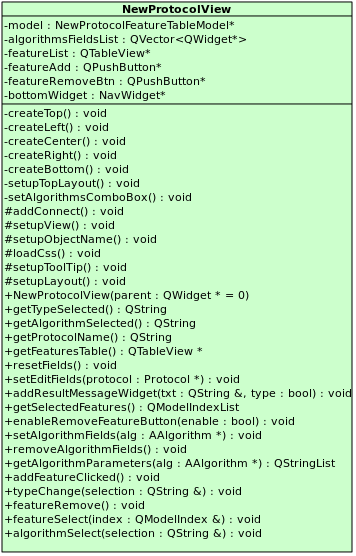
\includegraphics[width=0.6\linewidth]{./Content/Immagini/view/NewProtocolView.png}
			\caption{Diagramma Classe NewProtocolView: attributi e metodi}
			\label{cl_nsproview}
\end{figure}
\paragraph{Descrizione \\}
Classe che rappresenta il widget per la creazione di un nuovo \protocol{}.
\paragraph{Utilizzo\\}
La classe implementerà i metodi virtuali puri della superclasse inoltre darà la possibilità all'utente di inserire il nome del \protocol{}, selezionare il tipo di immagine a cui il protocol\g{} verrà applicato, potrà selezionare i Feature Extractors\g{} di interesse, settando i parametri richiesti lasciando opzionalmente quelli presenti di default, e/o selezionare uno e uno solo algoritmo di clastering\g{} comportandosi allo stesso modo per i Feature Extractors\g{}. Può poi proseguire al salvataggio del Protocol\g{} creato.
\paragraph{Classi ereditate\\}
\begin{itemize}
\item Window::APanel.
\end{itemize}
%%%%%%%ATTRIBUTI%%%%%%%%%%%
\paragraph{\textcolor{black}{Attributi\\}}
\begin{itemize}
\item\color{teal}\verb!-featureAdd: QPushButton*!
\color{black}
\subparagraph{Descrizione:} Pulsante che permette di aggiungere una nuova feature, da inserire nel Protocol in creazione.

%model
\item\color{teal}\verb!-model: NewProtocolFeatureTabelModel*!
\color{black}
\subparagraph{Descrizione:}
Modello che contiene la lista delle Feature fino a questo momento inserite nel \protocol{} in creazione.
%model
\item\color{teal}\verb!- algorithmFieldsList : QVector<QWidget*>!
\color{black}
\subparagraph{Descrizione:}
Vettore che contiene i puntatori ai campi degll'algoritmo.

%featureList
\item\color{teal}\verb!-featureList: QTabelView*!
\color{black}
\subparagraph{Descrizione:}contiene la lista delle Feature\g{} contenute dentro a \emph{model}. 

%algorith combo box
\item\color{teal}\verb!-algorithmCombobox: QComboBox*!
\color{black}
\subparagraph{Descrizione:}contiene la lista degli algoritmi di clustering\g{} presenti nell'applicativo \project{}. 

%name line edit
\item\color{teal}\verb!-nameLineEdit: QLineEdit*!
\color{black}
\subparagraph{Descrizione:}Linea di testa utilizzata per inserire il nome del \protocol{} che si sta creando. 

%type combo box
\item\color{teal}\verb!-typeComboBox: QComboBox*!
\color{black}
\subparagraph{Descrizione:}contiene la lista dei tipi di immagine a cui il \protocol{} verrà applicato. Una volta selezionato un tipo, verranno rese disponibili solo le Feature\g{} applicabili al tipo di immagine scelto.
\end{itemize}

%%%%%%%%%%%% METODI %%%%%%%%%%%
\paragraph{\textcolor{black}{Metodi\\}}
\begin{itemize}
%costruttore
\item \color{blue}\verb! + NewProtocolView(parent : QWidget*=0)!
\color{black}
\subparagraph{Descrizione:}
Costruttore per la classe NewSubjectView.
\subparagraph{Argomenti:}
\begin{itemize}
\item \color{RoyalPurple}\verb!parent: QWidget*=0 ! \\ Puntatore al QWidget padre di NewSubjectView.
\end{itemize}

%setupLayout()
\item \color{blue}\verb! #setupLayout():void!
\color{black} 
\subparagraph{Descrizione:}Metodo che implementa il contratto fornito dalla classe astratta \hyperref[speAPanel]{APanel}.
\subparagraph{Note:}
\begin{itemize}
\item questo metodo deve essere marcato virtuale;
\item questo metodo è stato ridefinito.
\end{itemize}

%setupToolTip
\item\color{blue}\verb! #setupToolTip():void!

\color{black}
\subparagraph{Descrizione:} Metodo che implementa il contratto fornito dalla classe astratta \hyperref[speAPanel]{APanel}.
 \subparagraph{Note:}
 \begin{itemize}
 \item questo metodo deve essere marcato virtuale;
 \item questo metodo è stato ridefinito.
 \end{itemize}
%createTop
\item \color{blue}\verb! -createTop():void!
\color{black}
\subparagraph{Descrizione:}Metodo che ha il compito di costruire la parte in alto del widget.

%createButtom
\item \color{blue}\verb! -createButtom():void!
\color{black}
\subparagraph{Descrizione:}Metodo che ha il compito di costruire la parte in basso del widget contenente il pulsante per ritornare alla pagine iniziale, il pulsante per il salvataggio e l'accesso alla guida.
 
%LOADCSS
\item \color{blue}\verb! #loadCss():void!
\color{black} 
\subparagraph{Descrizione:}Metodo che implementa il contratto fornito dalla classe astratta \hyperref[speAPanel]{APanel}.
 \subparagraph{Note}
 \begin{itemize}
  \item questo metododeve essere marcato virtuale;
 \item questo metodo è stato ridefinito.
 \end{itemize}

%setupObjectName
\item\color{blue}\verb! #setupObjectName():void!
\color{black}
\subparagraph{Descrizione:}Metodo che implementa il contratto fornito dalla classe astratta \hyperref[speAPanel]{APanel}.
 \subparagraph{Note}
 \begin{itemize}
  \item questo deve essere marcato virtuale;
 \item questo metodo è stato ridefinito.
 \end{itemize}

%addConnect
\item \color{blue}\verb! #addConnect():void!
\color{black}
\subparagraph{Descrizione:} Metodo che implementa il contratto fornito dalla classe astratta \hyperref[speAPanel]{APanel}.
 \subparagraph{Note}
 \begin{itemize}
 \item questo metodo deve essere marcato costante;
 \item questo metodo deve essere marcato virtuale;
 \item questo metodo è stato ridefinito.
 \end{itemize}

%setupView
\item \color{blue}\verb! #setupView():void!
\color{black}
\subparagraph{Descrizione:} Metodo che implementa il contratto fornito dalla classe astratta \hyperref[speAPanel]{APanel}.
 \subparagraph{Note}
 \begin{itemize}
 \item questo metodo deve essere marcato virtuale;
 \item questo metodo è stato ridefinito.
 \end{itemize}
%getTypeSelected
\item \color{blue}\verb! +getTypeSelected():QString!
\color{black} 
\subparagraph{Descrizione: }Metodo che ritorna il tipo a cui verrà applicato il protocol\g{}.
 \subparagraph{Note}
 \begin{itemize}
 \item questo metodo deve essere marcato costante.
 \end{itemize}
 
%getAlgorithmSelected
\item \color{blue}\verb! +getAlgorithmSelected():QString!
\color{black} 
\subparagraph{Descrizione:}Metodo che ritorna il nome dell'algoritmo selezionato.
 \subparagraph{Note}
 \begin{itemize}
 \item questo metodo deve essere marcato costante.
 \end{itemize}

%getprotocolName
\item \color{blue}\verb! +getProtocolName():QString!
\color{black}
\subparagraph{Descrizione:} Metodo che ritorna il nome da associare al nuovo \protocol{}.
 \subparagraph{Note}
 \begin{itemize}
 \item questo metodo deve essere marcato costante.
 \end{itemize}

%getFeaturesTable
\item \color{blue}\verb! +getFeaturesTable():QString!
\color{black} 
\subparagraph{Descrizione:}Metodo che ritorna la tabella contenente le features impostate.
 \subparagraph{Note}
 \begin{itemize}
 \item questo metodo deve essere marcato costante.
 \end{itemize}

%resetFields
\item \color{blue}\verb! +resetFields(): void!
\color{black}
\subparagraph{Descrizione:} Metodo che ripulisce i campi e li setta alle opzioni di predefinite.

%create left
\item \color{blue}\verb! -createLeft(): void!
\color{black}
\subparagraph{Descrizione:}Metodo che crea il layout per la parte sinistra della finestra contenente il nome da dare al nuovo protocol\g{} e il tipo di immagine a cui il protocol\g{} verrà applicato.

%createright
\item \color{blue}\verb! -createRight(): void!
\color{black} 
\subparagraph{Descrizione:}Metodo che crea il layout per la parte destra della finestra contenente le opzioni per l'inserimento dell'algoritmo di clustering\g{}.

%createCenter
\item \color{blue}\verb! -createCenter(): void!
\color{black} 
\subparagraph{Descrizione:}Metodo che crea il layout per la parte centrale della finestra contenente le opzioni per l'inserimento delle feature\g{}.

%setupTopLayout
\item \color{blue}\verb! -setupTopLayout(): void!
\color{black}
\subparagraph{Descrizione:} Metodo che imposta il layout della parte alta della finestra contenente le parti: destra, sinistra e centrale create dai metodi precedentemente illustrati.

%setEditableField
\item\color{blue}\verb! + setEditableFields(protocol: Protocol*):void!
\color{black} 
\subparagraph{Descrizione:}
Metodo che ha il compito di impostare i campi della view con i valori.
\subparagraph{Argomenti:}
\begin{itemize}
\item \color{RoyalPurple}\verb!protocol: Protocol* ! \\Rappresenta il \protocol{} da editare.
\end{itemize}

%addResultMessag
\item \color{blue} \verb! + addResultMessageWidget(txt: const QString\&, type: bool):void! 
\color{black}
\subparagraph{Descrizione:} Metodo che ha il compito di aggiungere il messaggio di risultato per avvenuta operazione o meno a seconda del valore del secondo parametro passato.
\subparagraph{Argomenti:}
\begin{itemize}
\item \color{RoyalPurple} \verb! txt: const QString\& ! \\Rappresenta il testo da mostrare all'utente all'interno del widget;
\item \color{RoyalPurple} \verb!type : bool ! \\ Vale true se il messaggio è un messaggio di successo, false se il messaggio è di errore.
\end{itemize}
\subparagraph{Note:}
\begin{itemize}
\item il metodo deve essere marcato virtuale.
\end{itemize}

%getSelectFeats
\item \color{blue} \verb! + getSelectedFeatures(): QModelIndexList! 
\color{black}
\subparagraph{Descrizione:} Metodo che ha il compito di ritornare  al Feature\g{} selezionata; ritorna una lista di indici di tabella.
\subparagraph{Note:}
\begin{itemize}
\item il metodo deve essere marcato costante.
\end{itemize}

%void enableRemoveFeatureButton(const bool enable)
\item \color{blue} \verb! + enableRemoveFeatureButton(enable: const bool): void!
\color{black}
\subparagraph{Descrizione:} Metodo che ha il compito di impostare la proprietà del pulsante abilitato o disabilitato, a seconda del valore del parametro passato.
\subparagraph{Argomenti:}
\begin{itemize}
\item \color{RoyalPurple} \verb! enable: const bool! \\ rappresenta il valore a cui impostare la proprietà del pulsante: true per abilitare il pulsante di rimozione della Feature\g{} false altrimenti.
\end{itemize}

%void setAlgorithmFields(AAlgorithm *alg)
\item \color{blue} \verb! + setAlgorithmFields(alg : AAlgorithm *) :void! 
\color{black}
\subparagraph{Descrizione:} Metodo che ha il compito di impostare i campi dei parametri dell'algoritmo.
\subparagraph{Argomenti:}
\begin{itemize}
\item \color{RoyalPurple} \verb! alg: AAlgorithm*! \\ rappresenta l'algoritmo di cui impostare i campi dei parametri.
\end{itemize}

%void removeAlgorithmFields()
\item \color{blue} \verb! + removeAlgorithmFields() :void! 
\color{black}
\subparagraph{Descrizione:} Metodo che ha il compito di rimuovere i campi dei parametri dell'algoritmo.


%void getAlgorithmParam(AAlgorithm *alg)const
\item \color{blue} \verb! + setAlgorithmFields(alg : AAlgorithm *) :void! 
\color{black}
\subparagraph{Descrizione:} Metodo che ha il compito di ritornare una lista contenente i valori dei parametri.
\subparagraph{Argomenti:}
\begin{itemize}
\item \color{RoyalPurple} \verb! alg: AAlgorithm*! \\ rappresenta l'algoritmo di cui cui ritornare il valore dei parametri.
\end{itemize}
\subparagraph{Note:}
\begin{itemize}
\item il metodo deve essere marcato come costante.
\end{itemize}

%%%%%%%%%%%%% signal
%addFeatureClicked
\item \color{blue}\verb! + addFeatureClicked():void! (signal)
\color{black} 
\subparagraph{Descrizione:}
Signal\g{} emesso quando l'utente decide di aggiungere una nuova Feature\g{} da calcolare al \protocol{}.

%typeChange(index:int)
\item\color{blue}\verb! + typeChange(index:int):void! (signal)
\color{black} 
\subparagraph{Descrizione:}
Signal\g{} emesso quando l'utente ha selezionato il tipo dalla combobox, servirà poi per poter mostrare all'utente solo le Feature\g{} disponibili per il tipo di immagine selezionato.
\subparagraph{Argomenti:}
\begin{itemize}
\item \color{RoyalPurple}\verb! index: int! \\rappresenta l'indice della voce selezionata dal menu a tendina.
\end{itemize}

%featRemove
\item \color{blue}\verb! + featureRemove():void! (signal)
\color{black} 
\subparagraph{Descrizione:}
Signal\g{} emesso quando l'utente preme il pulsante per la rimozione di una Feature\g{}.

%featSelect(index:QModelIndex\&)
\item\color{blue}\verb! + featureSelect(index:const QModelIndex \&):void! (signal)
\color{black} 
\subparagraph{Descrizione:}
Signal\g{} emesso quando l'utente seleziona un elemento dalla tabella.
\subparagraph{Argomenti:}
\begin{itemize}
\item \color{RoyalPurple}\verb! index: const QModelIndex\& ! \\rappresenta l'indice della tabella.
\end{itemize}

%featSelect(index:QModelIndex\&)
\item\color{blue}\verb! + AlgorithmSelect(selection:const QString \&):void! (signal)
\color{black} 
\subparagraph{Descrizione:}
Signal\g{} emesso quando l'utente seleziona un algoritmo.
\subparagraph{Argomenti:}
\begin{itemize}
\item \color{RoyalPurple}\verb! selection: const QString\&  ! \\rappresenta l'indice della tabella.
\end{itemize}

\end{itemize}
\color{black}
\pagebreak
%%%%%%%%%%%%%%%%%%%%%%%%%%%%%%%%%%%%%%%
%		NEWDatasetVIEW
%%%%%%%%%%%%%%%%%%%%%%%%%%%%%%%%%%%%%%%
\subsubsection{NewDatasetView (class)}
\label{speNdatV}
\begin{figure}[!h]
\centering
			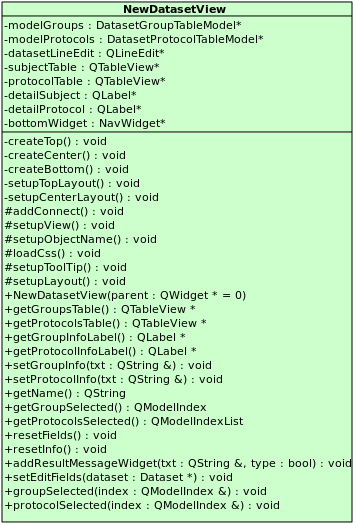
\includegraphics[width=0.5\linewidth]{./Content/Immagini/view/NewDatasetView.png}
			\caption{ Diagramma Classe NewDatasetView: attributi e metodi}
			\label{cl_ndatview}
\end{figure}
\paragraph{Descrizione \\}
Classe che rappresenta il widget per la creazione di un nuovo \dataset{}.
\paragraph{Utilizzo\\}
La classe implementerà i metodi virtuali puri della superclasse inoltre darà la possibilità all'utente di inserire un gruppo di \subject{} precedentemente creato, selezionare uno o più protocol\g{} da eseguire per quel gruppo di \subject{} e infine salvarlo.
\paragraph{Classi ereditate\\}
\begin{itemize}
\item Window::APanel.
\end{itemize}
%%%%%%%ATTRIBUTI%%%%%%%%%%%
\paragraph{\textcolor{black}{Attributi\\}}
\begin{itemize}
\item\color{teal}\verb!-datasetLineEdit: QLineEdit*!
\color{black}
\subparagraph{Descrizione:}Linea di testo che conterrà il nome del \dataset{} che l'utente sta andando a creare.
 
%modelGroups
\item\color{teal}\verb!-modelGroups: DatasetGroupTableModel*!
\color{black}
\subparagraph{Descrizione:}Modello per la tabella dei \subject{}.
 
%modelProtocol
\item\color{teal}\verb!-modelProtocols: DatasetProtocolTableModel*!
\color{black}
\subparagraph{Descrizione:}Modello che contiene tutti i \protocol{} che
 
%detailSubject
\item\color{teal}\verb!-detailSubject: QLabel*!
\color{black}
\subparagraph{Descrizione:}Contiene tutte le informazioni relative al \subject{} selezionato.
 
%protocolTable
\item\color{teal}\verb!-ProtocolTable: QTableView*!
\color{black}
\subparagraph{Descrizione:}Contiene la lista dei \protocol{} contenuti dentro a \emph{modelProtocols}
 
%subjectTable
\item\color{teal}\verb!-detailProtocol: QTableView*!
\color{black}
\subparagraph{Descrizione:}Contiene tutte le informazioni relative al \protocol{} selezionato.
 
%bottomWidget
\item\color{teal}\verb! bottomWidget:NavWidget*!
\color{black} 
 \subparagraph{Descrizione:}
Puntatore al widget che rappresenta la parte bassa della finestra contentente i pulsanti necessari al salvataggio all'annullamento delle operazioni e tornare indietro.
 \end{itemize}
%%%%%%%%%%%% METODI %%%%%%%%%%%
\paragraph{\textcolor{black}{Metodi\\}}
\begin{itemize}
%costruttore
\item\color{blue}\verb! + NewDatasetView(parent : QWidget*=0)!
\color{black}
\subparagraph{Descrizione:}Costruttore per la classe NewDatasetView.
\subparagraph{Argomenti:}
\begin{itemize}
\item \color{RoyalPurple}\verb!parent: QWidget*=0 ! \\ Puntatore al QWidget padre di NewDatasetView.
\end{itemize}
 
%setupToolTip
\item\color{blue}\verb! #setupToolTip():void!

\color{black}
\subparagraph{Descrizione:} Metodo che implementa il contratto fornito dalla classe astratta \hyperref[speAPanel]{APanel}.
 \subparagraph{Note:}
 \begin{itemize}
 \item questo metodo deve essere marcato virtuale;
 \item questo metodo è stato ridefinito.
 \end{itemize} 
 
%setupLayout()
\item\color{blue}\verb! #setupLayout():void!
\color{black} 
\subparagraph{Descrizione:}Metodo che implementa il contratto fornito dalla classe astratta \hyperref[speAPanel]{APanel}.
\subparagraph{Note:}
\begin{itemize}
\item questo metodo deve essere marcato virtuale;
\item questo metodo è stato ridefinito.
\end{itemize}
  
%createTop
\item\color{blue}\verb! -createTop():void!
\color{black}
\subparagraph{Descrizione:} Metodo che ha il compito di costruire la parte in alto del widget contenente la form per l'inserimento dei dati necessari per la creazione di un nuovo \dataset{}.
  
%createCenter
\item\color{blue}\verb! -createCenter():void!
\color{black} 
\subparagraph{Descrizione:}Metodo che ha il compito di costruire la parte centrale del widget per la vista che si occupa della  creazione di un nuovo \dataset{}.
  
%createButtom
\item\color{blue}\verb! -createButtom():void!
\color{black} 
\subparagraph{Descrizione:}Metodo che ha il compito di costruire la parte in basso del widget contenente il pulsante per ritornare alla pagine iniziale, il pulsante per il salvataggio e l'accesso alla guida.
 
%setupTopLayout
\item\color{blue}\verb! -setupTopLayout():void!
\color{black} 
\subparagraph{Descrizione:}Metodo che ha il compito di impostare la parte alta del layout della finestra.
   
%setupCenterLayout()
\item\color{blue}\verb! -setupCenterLayout():void!
\color{black} 
\subparagraph{Descrizione:}Metodo che ha il compito di impostare la parte centrale del layout della finestra.
  
%LOADCSS
\item\color{blue}\verb! #loadCss():void!
\color{black}
\subparagraph{Descrizione:} Metodo che implementa il contratto fornito dalla classe astratta \hyperref[speAPanel]{APanel}.
 \subparagraph{Note:}
 \begin{itemize}
  \item questo metododeve essere marcato virtuale;
 \item questo metodo è stato ridefinito.
 \end{itemize}
  
%setupObjectName
\item\color{blue}\verb! #setupObjectName():void!
\color{black}
\subparagraph{Descrizione:}Metodo che implementa il contratto fornito dalla classe astratta \hyperref[speAPanel]{APanel}.
 \subparagraph{Note:}
 \begin{itemize}
  \item questo deve essere marcato virtuale;
 \item questo metodo è stato ridefinito.
 \end{itemize}
  
%addConnect
\item\color{blue}\verb! #addConnect():void!
\color{black}
\subparagraph{Descrizione:}Metodo che implementa il contratto fornito dalla classe astratta \hyperref[speAPanel]{APanel}.
 \subparagraph{Note:}
 \begin{itemize}
 \item questo metodo deve essere marcato costante;
 \item questo metodo deve essere marcato virtuale;
 \item questo metodo è stato ridefinito.
 \end{itemize}
  
%setupView
\item\color{blue}\verb! #setupView():void!
\color{black}
\subparagraph{Descrizione:}Metodo che implementa il contratto fornito dalla classe astratta \hyperref[speAPanel]{APanel}.
 \subparagraph{Note:}
 \begin{itemize}
 \item questo metodo deve essere marcato virtuale;
 \item questo metodo è stato ridefinito.
 \end{itemize}
 
%getGroupTable
\item\color{blue}\verb! +getGroupTable(): QTableView*!
\color{black} 
\subparagraph{Descrizione:}Metodo che ritorna la lista dei gruppi di \subject{} disponibili.
 \subparagraph{Note:}
 \begin{itemize}
 \item questo metodo deve essere marcato costante.
 \end{itemize}
 
%getProtocTable
\item\color{blue}\verb! +getProtocolsTable(): QTableView*!
\color{black} 
\subparagraph{Descrizione:}Metodo che ritorna la lista dei \protocol{} disponibili.
 \subparagraph{Note:}
 \begin{itemize}
 \item questo metodo deve essere marcato costante.
 \end{itemize}
%getName
\item\color{blue}\verb! +getName(): QString!
\color{black} 
\subparagraph{Descrizione:}Metodo che ritorna il nome del \dataset{}.  
 \subparagraph{Note:}
 \begin{itemize}
 \item questo metodo deve essere marcato costante.
 \end{itemize}
  
%get groupSelect
\item\color{blue}\verb! +getGroupSelected(): QModelIndex*!
\color{black} 
\subparagraph{Descrizione:}Metodo che ritorna un indice di tabella del gruppo selezionato.  
 \subparagraph{Note:}
 \begin{itemize}
 \item questo metodo deve essere marcato costante.
 \end{itemize}
 
%get protoSelect
\item\color{blue}\verb! +getProtocolsSelected(): QModelIndex*!
\color{black} 
\subparagraph{Descrizione:}Metodo che ritorna un indice di tabella del \protocol{}selezionato.  
 \subparagraph{Note:}
 \begin{itemize}
 \item questo metodo deve essere marcato costante.
 \end{itemize} 
  
%resetInfo
\item\color{blue}\verb! + resetInfo(): void!
\color{black} 
\subparagraph{Descrizione:}Metodo che reimposta il box delle informazioni.

%resetFields
\item\color{blue}\verb! + resetFields(): void!
\color{black} 
\subparagraph{Descrizione:}Metodo che reimposta tutti i campi della view.    

%getgroup
\item\color{blue}\verb! +getGroupInfoLabel(): QLabel*!
\color{black} 
\subparagraph{Descrizione:}Metodo che ritorna una label contenenente le informazioni relative al gruppo selezionato.  
 \subparagraph{Note:}
 \begin{itemize}
 \item questo metodo deve essere marcato costante.
 \end{itemize}
 
%getProto
\item\color{blue}\verb! +getProtocolInfoLabel(): QLabel*!
\color{black} 
\subparagraph{Descrizione:}Metodo che ritorna una label contenenente le informazioni relative al \protocol{} selezionato.  
 \subparagraph{Note:}
 \begin{itemize}
 \item questo metodo deve essere marcato costante.
 \end{itemize}
 
%setProtocolInfo
\item\color{blue}\verb! +setProtocolInfo(txt: QString\&): void!
\color{black}
\subparagraph{Descrizione:} Metodo che imposta le informazioni del protocol selezionato.  
 \subparagraph{Argomenti:}
 \begin{itemize}
 \item \color{RoyalPurple} \verb!txt: QString\& !\\ txt contiene il testo che verrà settato per il capo dati \emph{detailProtocol}.
 \end{itemize}
 
%setGroupInfo
\item\color{blue}\verb! +setGroupInfo(txt: QString\&): void!
\color{black}
\subparagraph{Descrizione:} Metodo che imposta le informazioni del gruppo selezionato.  
 \subparagraph{Argomenti:}
 \begin{itemize}
 \item \color{RoyalPurple} \verb!txt: QString\& !\\ txt contiene il testo che verrà settato per il capo dati \emph{detailsSubject}.
 \end{itemize}
 
%seteditFields
\item\color{blue}\verb! +setEditFields(dataset: Dataset*): void!
\color{black}
\subparagraph{Descrizione:} Metodo che imposta i campi con i dati.  
 \subparagraph{Argomenti:}
 \begin{itemize}
 \item \color{RoyalPurple} \verb!dataset: Dataset* !\\ Rappresenta il puntatore al \dataset{} da editare.
 \end{itemize} 
 
 %addResultMessag
\item \color{blue} \verb! + addResultMessageWidget(txt: const QString\&, type: bool):void! 
\color{black}
\subparagraph{Descrizione:} Metodo che ha il compito di aggiungere il messaggio di risultato per avvenuta operazione o meno a seconda del valore del secondo parametro passato.
\subparagraph{Argomenti:}
\begin{itemize}
\item \color{RoyalPurple} \verb! txt: const QString\& ! \\Rappresenta il testo da mostrare all'utente all'interno del widget;
\item \color{RoyalPurple} \verb!type : bool ! \\ Vale true se il messaggio è un messaggio di successo, false se il messaggio è di errore.
\end{itemize}
\subparagraph{Note:}
\begin{itemize}
\item il metodo deve essere marcato virtuale.
\end{itemize}


%%%%%%%%%%%% signal
%groupSelected
\item\color{blue}\verb! +groupSelected(index:QModelIndex\&):void! (signal)
\color{black} 
\subparagraph{Descrizione:}
Signal\g{} emesso quando l'utente seleziona un gruppo dalla tabella identificata dal campo dati \emph{subjectTable}.
 
%protocolSelect
\item\color{blue}\verb! +groupSelected(index:QModelIndex\&):void! (signal)
\color{black} 
 \subparagraph{Descrizione:}
Signal\g{} emesso quando l'utente seleziona un \protocol{} dalla tabella identificata dal campo dati \emph{protocolTable}.
 \end{itemize}
\pagebreak
\color{black}
%%%%%%%%%%%%%%%%%%%%%%%%%%%%%%%%%%
%		SUBJECTSVIEW
%%%%%%%%%%%%%%%%%%%%%%%%%%%%%%%%%%
\subsubsection{SubjectsView (class)}
\label{spesubV}
\begin{figure}[!h]
\centering
			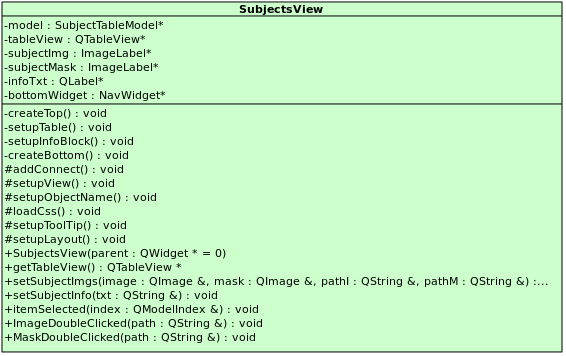
\includegraphics[width=0.75\linewidth]{./Content/Immagini/view/SubjectsView.png}
			\caption{Diagramma Classe SubjectsView: attributi e metodi}
			\label{cl_subview}
\end{figure}
\paragraph{Descrizione \\}
Classe che rappresenta il widget per la visualizzazione di tutti i \subject{} presenti all'interno di \project.
\paragraph{Utilizzo\\}
La classe implementerà i metodi virtuali puri della superclasse inoltre darà la possibilità all'utente di visualizzare l'elenco di tutti i \subject{} fino a quel momento creati e memorizzati dentro a \project. Selezionando un \subject{} sarà possibile visualizzare le informazioni relative a quel \subject{}.
\paragraph{Classi ereditate\\}
\begin{itemize}
\item Window::APanel.
\end{itemize}
%%%%%%%ATTRIBUTI%%%%%%%%%%%
\paragraph{\textcolor{black}{Attributi\\}}
\begin{itemize}
\item\color{teal}\verb!-model: SubjectTableModel *!

\color{black}Modello che contiene i \subject presenti nel sistema.

%tabelView
\item\color{teal}\verb!-tableView: QTabelView*!
\color{black}

Contiene la lista dei \subject contenuti nel campo dati \emph{model}.

%subjImg
\item\color{teal}\verb!-subjectImg: QLabel*!
\color{black}

Contiene l'immagine relativa al subject\g{} selezionato.

%subjmask
\item\color{teal}\verb!-subjectMask: QLabel*!

\color{black}
Contiene la maschera relativa al subject\g{} selezionato.

%infoTxt
\item\color{teal}\verb!-infoTxt: QLabel*!

\color{black}
Contiene le informazioni relative al \subject{} selezionato.

%bottomWidget
\item\color{teal}\verb! bottomWidget:NavWidget*!
\color{black} 

Puntatore al widget che rappresenta la parte bassa della finestra contentente i pulsanti per tornare indietro e per la visualizzazione della guida interattiva.
\end{itemize}
%%%%%%%%%  METODI
\paragraph{\textcolor{black}{Metodi\\}}
\begin{itemize}
%costruttore
\item\color{blue}\verb! + SubjectsView(parent : QWidget*=0)!
\color{black}
\subparagraph{Descrizione: }Costruttore per la classe SubjectsView. 
\subparagraph{Argomenti:}
\begin{itemize}
\item \color{RoyalPurple}\verb!parent: QWidget*=0 ! \\ Puntatore al QWidget padre di SubjectsView.
\end{itemize}

%setupLayout()
\item\color{blue}\verb! #setupLayout():void!
\color{black} 
\subparagraph{Descrizione: }Metodo che implementa il contratto fornito dalla classe astratta \hyperref[speAPanel]{APanel}.
\subparagraph{Note: }
\begin{itemize}
\item questo metodo deve essere marcato virtuale;
\item questo metodo è stato ridefinito.
\end{itemize}
 
%createTop
\item\color{blue}\verb! -createTop():void!
\color{black} 
\subparagraph{Descrizione: }Metodo che ha il compito di costruire la parte in alto del widget contenente l'elenco dei \subject e a lato lo spazio per visualizzare le informazioni.
 
%createButtom
\item\color{blue}\verb! -createButtom():void!
\color{black}
\subparagraph{Descrizione: } Metodo che ha il compito di costruire la parte in basso del widget contenente il pulsante per ritornare alla pagine iniziale, e per l'accesso alla guida.

%setupTable
%createButtom
\item\color{blue}\verb! -setupTable():void!
\color{black}
\subparagraph{Descrizione: } Metodo che ha il compito di impostare la tabella che visualizzerà l'elenco dei \subject{} presenti nel sistema.

%createButtom
\item\color{blue}\verb! -setupInfoBlock():void!
\color{black}
\subparagraph{Descrizione: } Metodo che ha il compito di impostare il layout riguardante la visualizzazione delle informazioni.

%LOADCSS
\item\color{blue}\verb! #loadCss():void!
\color{black} 
\subparagraph{Descrizione: }Metodo che implementa il contratto fornito dalla classe astratta \hyperref[speAPanel]{APanel}.
 \subparagraph{Note:}
 \begin{itemize}
  \item questo metododeve essere marcato virtuale;
 \item questo metodo è stato ridefinito.
 \end{itemize}
 
%setupObjectName
\item\color{blue}\verb! #setupObjectName():void!
\color{black}
\subparagraph{Descrizione: }Metodo che implementa il contratto fornito dalla classe astratta \hyperref[speAPanel]{APanel}.
 \subparagraph{Note:}
 \begin{itemize}
  \item questo deve essere marcato virtuale;
 \item questo metodo è stato ridefinito.
 \end{itemize}
 
%setupToolTip
\item\color{blue}\verb! #setupToolTip():void!
\color{black}
\subparagraph{Descrizione: }Metodo che implementa il contratto fornito dalla classe astratta \hyperref[speAPanel]{APanel}.
 \subparagraph{Note:}
 \begin{itemize}
 \item questo metodo deve essere marcato virtuale;
 \item questo metodo è stato ridefinito.
 \end{itemize}
 
%addConnect
\item\color{blue}\verb! #addConnect():void!
\color{black}
\subparagraph{Descrizione: }Metodo che implementa il contratto fornito dalla classe astratta \hyperref[speAPanel]{APanel}.
 \subparagraph{Note:}
 \begin{itemize}
 \item questo metodo deve essere marcato costante;
 \item questo metodo deve essere marcato virtuale;
 \item questo metodo è stato ridefinito.
 \end{itemize}
 
%setupView
\item\color{blue}\verb! #setupView():void!
\color{black}
\subparagraph{Descrizione: }Metodo che implementa il contratto fornito dalla classe astratta \hyperref[speAPanel]{APanel}.
 \subparagraph{Note:}
 \begin{itemize}
 \item questo metodo deve essere marcato virtuale;
 \item questo metodo è stato ridefinito.
 \end{itemize}

%subjView
\item\color{blue}\verb! -getTableView():QTabelView*!
\color{black}
Metodo che ritorna il puntatore campo dati \emph{tableView}.
 \subparagraph{Note:}
 \begin{itemize}
 \item questo metodo deve essere marcato costante.
 \end{itemize}

%setsubjImg
\item\color{blue}\verb! -setSubjectImg(imgage:QImage&):void!
\color{black}
\subparagraph{Descrizione: }Metodo che imposta l'immagine del \subject{} nella parte delle informazioni relative al \subject{}.
\subparagraph{Argomenti:}
\begin{itemize}
\item \color{RoyalPurple}\verb!image: QImage& !\\ contiene l'immagine che verrà impostata nella parte delle informazioni.
\end{itemize}

%setsubjmask
\item\color{blue}\verb! -setSubjectMask(imgage:QImage&):void!
\color{black}
\subparagraph{Descrizione: }Metodo che imposta la maschera del \subject{} nella parte delle informazioni relative al \subject{}.
\subparagraph{Argomenti:}
\begin{itemize}
\item \color{RoyalPurple}\verb!image: QImage& !\\ contiene la maschera che verrà impostata nella parte delle informazioni.
\end{itemize}

%setSubjectInfo
\item\color{blue}\verb! -setSubjectInfo(txt:QString&):void!
\color{black}
\subparagraph{Descrizione: }Metodo che imposta tutte le informazioni del \subject selezionato nella parte deidicata alle informazioni.
\subparagraph{Argomenti:}
\begin{itemize}
\item \color{RoyalPurple}\verb!txt: QString& !\\ stringa contenente le nuove informazioni da visualizzare.
\end{itemize}

%itemSelected
\item\color{blue}\verb! +itemSelected(index:QModelIndex&):void! (signal)
\color{black} 
\subparagraph{Descrizione: }
Signal\g{} emesso quando l'utente seleziona un \subject{} dalla tabella contenente tutti i \subject{} presenti.
\subparagraph{Attributi:}
\begin{itemize}
\item \color{RoyalPurple}\verb! index: QModelIndex& ! \\ rappresenta l'indice della tabella selezionato.
\end{itemize}

%setSubjectInfo
\item\color{blue}\verb! + imageDoubleClicked(path:const QString&):void! (signal)
\color{black}
\subparagraph{Descrizione: }
Signal\g{} emesso quando l'utente seleziona con un doppio click sull'immagine del \subject{}.
\subparagraph{Argomenti:}
\begin{itemize}
\item \color{RoyalPurple}\verb!path: QString& !\\ stringa contenente il path relativo all'immagine.
\end{itemize}

%smaskdouble
\item\color{blue}\verb! + maskDoubleClicked(path:const QString&):void!(signal)
\color{black}
\subparagraph{Descrizione: }
Signal\g{} emesso quando l'utente seleziona con un doppio click la maschera associata all'immagine del \subject{}.
\subparagraph{Argomenti:}
\begin{itemize}
\item \color{RoyalPurple}\verb!path: QString& !\\ stringa contenente il path relativo all'immagine.
\end{itemize}
\end{itemize}
\pagebreak
\color{black}